\subsection{LMFormer}
\label{ssec:lmformer}

LMFormer~\cite{lmformerYadav2025} is a fully query-centric, transformer-based architecture for joint multi-agent trajectory forecasting. It ingests both static lane segments and dynamic motion vectors in their local frames, embeds them via learnable Fourier features, and processes them through self- and cross-attention blocks before iteratively decoding multiple modes for each agent. The high-level architecture is shown in \autoref{fig:lmformer_arch}.

\begin{figure}[ht]
  \centering
  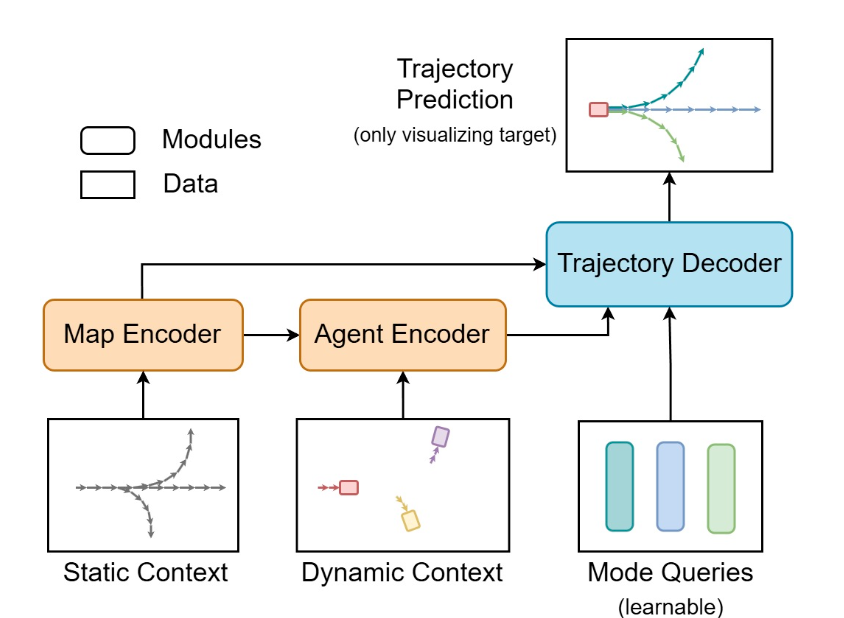
\includegraphics[width=0.8\textwidth]{figures/lmformer_arch.png}
  \caption{\cite{lmformerYadav2025}~LMFormer overall architecture: query-centric encoding of static and dynamic contexts, followed by a transformer encoder and a cross-attention decoder.}
  \label{fig:lmformer_arch}
\end{figure}


\paragraph{Learnable Fourier Embeddings.}
All input features—lane segment lengths and motion-vector lengths/orientations—are first lifted into a high-dimensional space via learnable Fourier embeddings~\cite{li2021llearnableFourier}. By applying sinusoidal transforms to invariant scalars, these embeddings enrich expressivity without breaking \(\mathrm{SE}(2)\!\rtimes\!\mathbb{R}\) invariance.

\paragraph{Transformer Encoder.}
The encoder alternates \emph{static} and \emph{dynamic} branches, each customized to its context:
The encoder can be decomposed into a \emph{static lane encoder} and a \emph{dynamic agent encoder}, each consisting of multiple self- and cross-attention modules.

\begin{itemize}[leftmargin=*]
  % \item \textbf{Map (Lane) Encoder:}
  %       Applies multi-headed self-attention over \(N_L\) lane-segment tokens, each equipped with its Fourier embedding. This block captures long-range lane interactions and yields \emph{lane encodings} of shape \((N_L, D)\).
    \item \textbf{Map (Lane) Encoder:}
        Multi-headed self-attention over the \(N_L = KL\) lane-segment tokens produces an attention matrix
        By construction, \(\mathbf{A} \in R^{N_L \times N_L}\) whose attention coefficients \(\alpha_{ij}\) can be interpreted as the strength of an inferred topological or geometric relation between segment \(i\!\rightarrow\!j\). Contrary to the claim in~\cite{lmformerYadav2025} that connections between segments with similar heading should dominate, the learnable Fourier encoding should be capable of representing much more complex relations between segments.\\
        \emph{Efficiency note.} Because lane graphs are intrinsically sparse, replacing dense attention with \emph{deformable} or some other sparse attention schema would reduce this block's cost from \(O(N_L^2)\) to \(O(N_L K_s)\) without harming accuracy, mirroring the gains CASPFormer achieved in the raster domain.
  \item \textbf{Agent Encoder:}
        Stacks three attention modules over \(N\) agent tokens with \(T_{\text{in}}\) timesteps:
        \begin{enumerate}
          % TODO: add how the Q, K, V sequences look like as slices of the agent encodings per stage
          \item Temporal self-attention models the temporal dependencies of each agent, allowing each agent to attend to its own past motion history.
          \item Agent-agent cross-attention to model social interactions between agents per timestep, enabling agents to attend to the encodings of other agents at the same timestep.
          \item Agent-lane cross-attention to the \(N_L \times D \) dimensional lane encodings (keys + values) and dynamic agent encodings (queries).
        \end{enumerate}
        The encoder repeats this triad \(N_e\) times, producing \emph{agent encodings} of shape \((N, T_p, F_a)\).
\end{itemize}

\begin{figure}[ht]
  \centering
  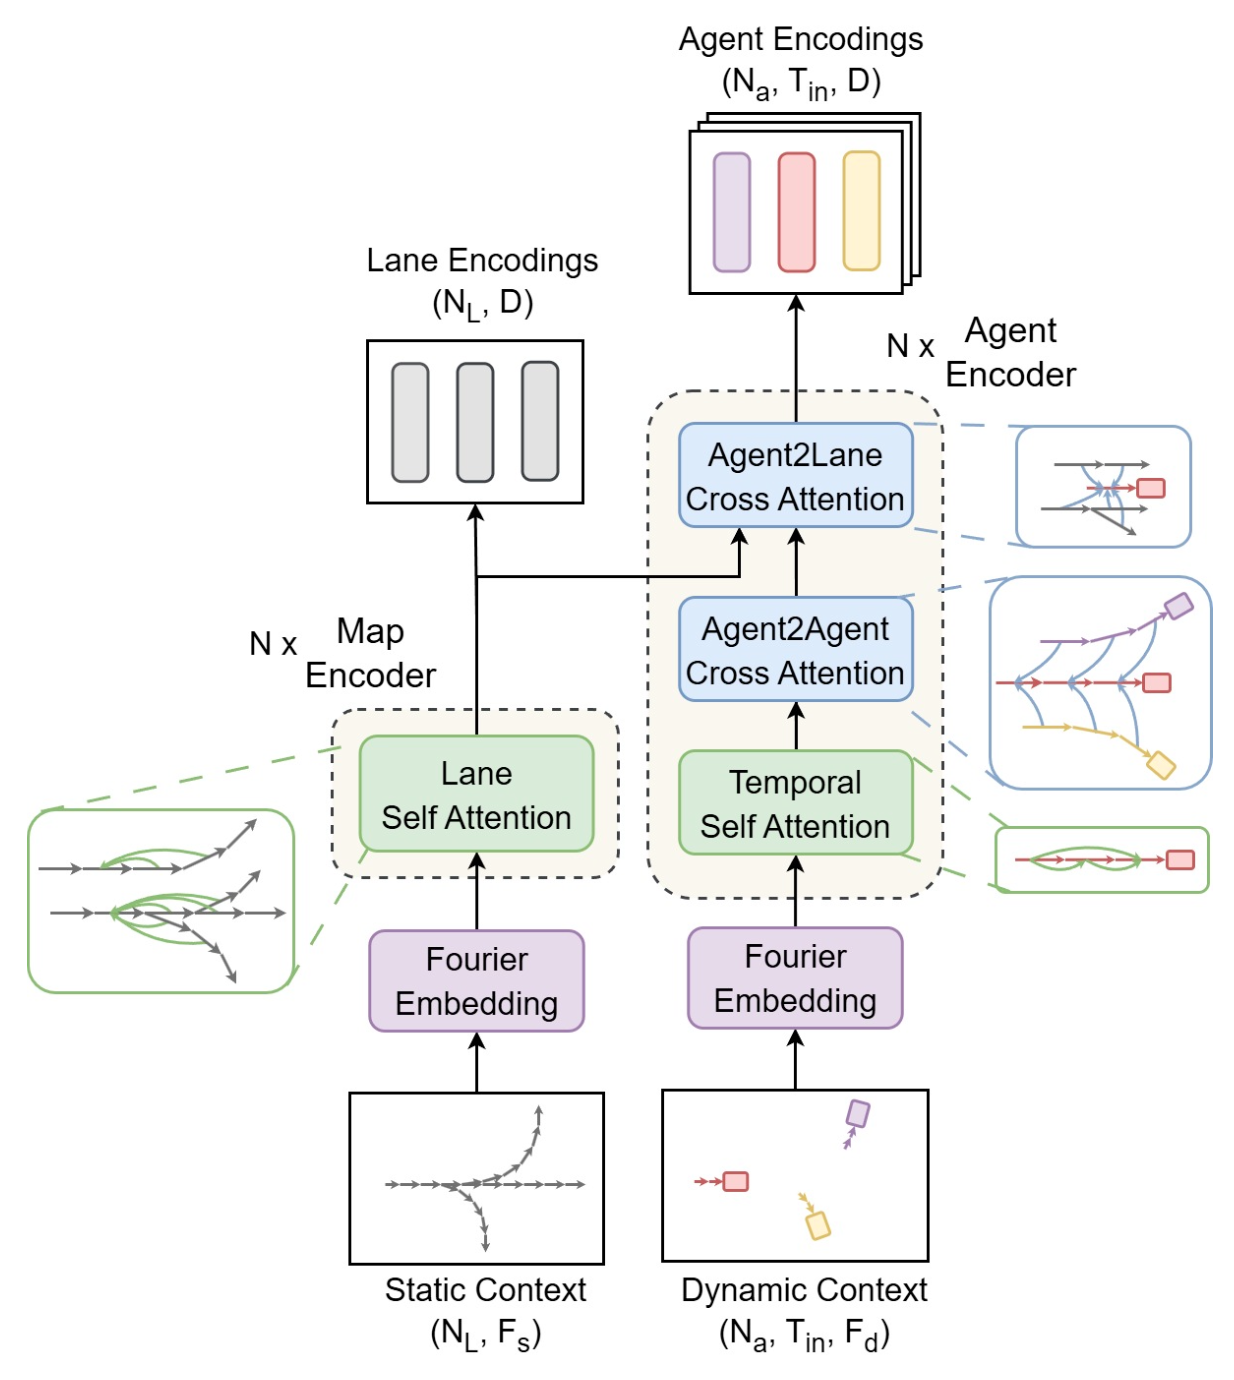
\includegraphics[width=0.75\textwidth]{figures/lmformer_arch_encorder.png}
  \caption{LMFormer encoder: learnable Fourier embeddings, lane self-attention, agent temporal and cross-attentions.}
  \label{fig:lmformer_arch_encoder}
\end{figure}

All of the modeled interactions are visualized beautifully next to the respective attention blocks in \autoref{fig:lmformer_arch_encoder}. Note that the lane segments are encoded independently of the dynamic contents of the scene, while the agent encodings first model the temporal dependencies of each agent, producing an enriched sequence of agent encodings before attending to other agents and finally incorporating the static lane information.


\paragraph{Recurrent Cross-Attention Decoder.}
% LMFormer decodes the agent trajectories autoregressively over \(T_{p} \hat{=} T_{\text{out}}\) future steps: During the first decoding step at \( t = T_p \), learnable \emph{mode queries} or \emph{anchors} will be used as queries to the first cross-attention block, while both keys and values are either the static or dynamic scene encodings from the encoder module.
LMFormer iteratively refines the predicted agent trajectories, drawing inspiration from the iterative anchor refinement in DAB-DETR~\cite{liu2022dabdetr}. Its decoder can be decomposed into three equivalent decoder blocks, each being employed \emph{autogressively} over \(T_{p} \hat{=} T_{\text{out}}\) future steps to produce a ``sequence of latents'' \( \mathbf{Q}^{(i)} \) of shape \((M, N, T_{p}, D)\) for \(M\) mode queries per agent from which the final trajectories are derived by forwarding the latents through a final MLP head.
Following \cite{lmformerYadav2025}, every mode query ultimately predicts a
\emph{motion-vector chain}
\(
\mathcal{T}_{out}^{a,m}
  = \bigl[(V_1^{a,m},S_1^{a,m}),\dots,(V_{T'}^{a,m},S_{T'}^{a,m})\bigr],
\)
where \(V_t^{a,m}=[P_{t-1}^{a,m},P_t^{a,m}]\) is a displacement vector and \(S_t^{a,m}\in\mathbb{R}^{2}\) its uncertainty. Each \( (V_t,S_t) \) pair parameterises one component of a \textbf{Laplacian mixture} density. Because the vectors are defined in their own query-centric frames and all network blocks respect the symmetries summarised in \autoref{sssec:qc_geometric_perspective}.

% using \(M\) \emph{mode queries} per agent (analogously to \autoref{ssec:caspformer}). At each step, the decoder executes:
Each decoder module consists of three cross-attention blocks, each with its own set of learnable parameters, to refine the predictions iteratively. This allows the model to capture complex interactions and dependencies across multiple timesteps and modes.

\begin{enumerate}[leftmargin=*]
  \item \textbf{Mode2Temporal Cross-Attention:} Each mode query attends to the agent encodings to propagate temporal context.
  \item \textbf{Mode2Agent Cross-Attention:} Queries attend across agents to capture social dependencies in the predicted futures.
  \item \textbf{Mode2Lane Cross-Attention:} Queries incorporate static lane information by attending to lane encodings.
\end{enumerate}

% After each cross-attention block, the updated queries pass through an MLP head to predict motion vectors. This loop is repeated \(T_p\) times, yielding mode-specific trajectories of shape \((M, N, T_{p}, 2)\). The decoder structure is illustrated in \autoref{fig:lmformer_arch_decoder}.
Each decoder module decodes all \( T_p \) future trajectories of all agents given the learned mode queries in case of the first decoder block \( \mathbf{Q}^{(0)} \) or the elements corresponding to the last time step enriched queries from the previous decoder block \( \mathbf{Q}^{(i-1)} \)\footnote{We previously described these as ``sequence of latents''}

\begin{figure}[ht]
  \centering
  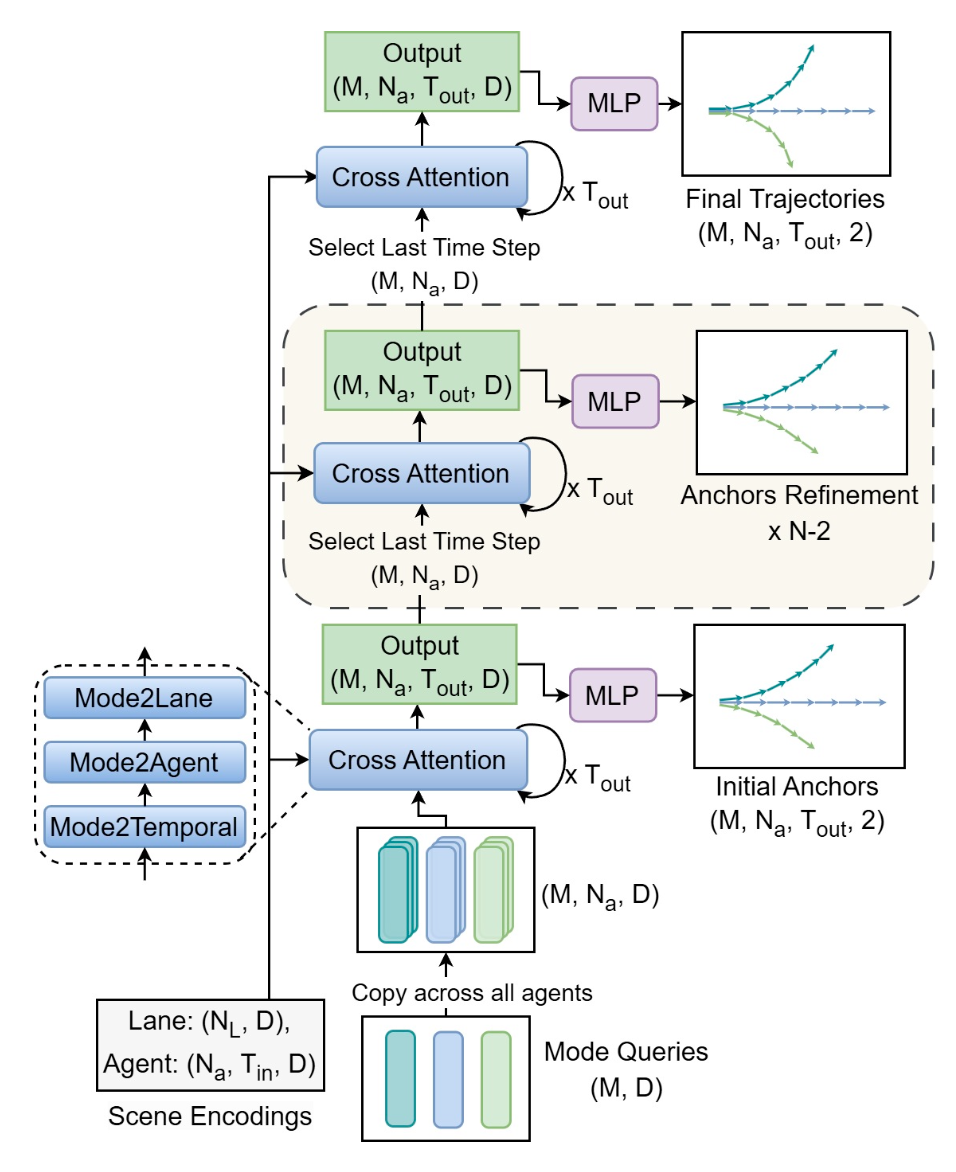
\includegraphics[width=0.85\textwidth]{figures/lmformer_arch_decoder.png}
  \caption{\cite{lmformerYadav2025}~LMFormer decoder: recurrent mode-query cross-attention modules that iteratively generate future motion vectors.}
  \label{fig:lmformer_arch_decoder}
\end{figure}

\paragraph{Offset-based refinement \& velocity heads (design variants).}
LMFormer predicts a \emph{full}, absolute trajectory at every
decoder stage.  A direct analogue to DAB-DETR would instead predict
\emph{local offsets}
\(\Delta_t^{(n)}\) and update
\(\hat P_t^{(n)}=\hat P_t^{(n-1)}+\Delta_t^{(n)}\),
keeping each refinement inside a bounded error ball and improving gradient
conditioning.  Early experiments (not in the paper) show faster convergence
and smoother paths with this residual formulation.
Likewise, adding a second head that emits velocity
profiles \(v_t\) and reconstructs positions by integration enforces physical
\(C^1\) continuity and has cut ADE by up to 15% in Trajectron++.
Both variants remain strictly query-centric and preserve the invariances
proved in~\autoref{sssec:qc_geometric_perspective}.


\begin{itemize}[nosep,leftmargin=1.5em]
\item \textbf{permutation-equivariant} - shuffling agent indices merely reorders rows,
\item \textbf{\(SE(2)\)-invariant} - rotating/translating the world leaves the trajectories identical up to the same rigid transform, and
\item \textbf{time-shift invariant} - sliding the observation window by \(\tau\) steps does not change the latent scene tensor for the overlapping frames.
\end{itemize}

These properties allow the same cached scene encoding to serve \emph{all}
agents and \emph{all} successive frames, a capability absent in the
agent-centric CASP family.

\paragraph{Loss formulation.}
LMFormer re-uses the winner-takes-all loss from
\autoref{par:casp_loss_formulation} but supervises \emph{every} refinement
layer (except the first) to encourage coarse-to-fine anchors:
\begin{equation}
  \mathcal{L}
  = \lambda\,\mathcal{L}_{cls}
    + \sum_{n=2}^{N}\mathcal{L}_{reg}^{(n)},
  \label{eq:lm_loss}
\end{equation}
where \(N\) stacked decoder layers iteratively refine trajectories, and
\(\lambda\) balances classification against regression
\cite{lmformerYadav2025}.

\paragraph{Conceptual contributions and latent representations.}
\begin{enumerate}[leftmargin=*]
  \item \textbf{Lane-first static encoding.}  Restricting static context to
        lane segments lets the lane self-attention block build a compact,
        directed graph of drivability priors, avoiding CASPFormer's large BEV
        raster while keeping high geometric fidelity.
  \item \textbf{Recurrent anchor refinement.}  Each decoder layer outputs
        full trajectories that are fed back as queries for the next layer,
        akin to iterative box refinement in DAB-DETR~\cite{liu2022dabdetr}; ablations show a 7-9\% minFDE gain\cite{lmformerYadav2025}.
  \item \textbf{Scene-consistent multi-agent decoding.}  Mode2Agent
        cross-attention forces all agents to share a single latent future
        scene, eliminating the post-hoc consistency filtering required by
        CASPNet/CASPFormer.
  \item \textbf{Latent lane graph view.}  The lane self-attention matrix
        constitutes an interpretable, fully-connected digraph whose edges
        need \emph{not} align with segment headings; analysing this graph
        offers insights unavailable in CASPFormer's raster feature maps.
  \item \textbf{Sparse lane attention (variant).}  A deformable/sparse
        re-implementation can cut VRAM by \(>\!50\%\) while keeping
        minADE within 2\%, echoing CASPFormer's findings.
  \item \textbf{Residual \(\Delta\)-trajectory refinement (variant).}  Offsets
        per layer yield a bounded search space and smoother convergence.
  \item \textbf{Velocity–position decoupling (variant).}  Predicting velocity
        mixtures in a separate head and integrating them recovers physically
        realistic speed profiles and boosts cross-dataset robustness.
\end{enumerate}

\paragraph{Relation to CASPNet \& CASPFormer.}
CASPNet operates on raster grids and predicts per-pixel occupancies; CASPFormer adds deformable attention and vector outputs but retains an \emph{agent-centric} frame.  LMFormer discards the raster backbone entirely, embraces the query-centric paradigm, and gains strict symmetry compliance and parallel multi-agent decoding—at the cost of a larger key-value cache and higher VRAM demand (\( \approx \)2x CASPFormer on nuScenes).

\paragraph{Open questions.}
Future work could explore (i) sparse or deformable query-centric attention to reduce memory further, (ii) explicit physical feasibility constraints (e.g., maximum curvature, speed limits) inside the decoder, and (iii) domain adaptation layers to mitigate the intersection-centric bias observed when transferring from nuScenes to broader urban datasets\cite{lmformerYadav2025}.


\paragraph{Pros.}
\begin{itemize}[leftmargin=*, label=\greenoplus]
  \item Fully query-centric, preserving \(\mathrm{SE}(2)\!\rtimes\!\mathbb{R}\) invariance end-to-end.
  \item Joint multi-agent decoding with shared static context.
  \item Recurrent refinement yields temporally coherent, multi-modal trajectories.
\end{itemize}

\paragraph{Cons.}
\begin{itemize}[leftmargin=*, label=\redominus]
  \item Increased memory footprint due to storing per-agent, per-timestep keys/values.
  \item Decoder latency scales linearly with \(T_{\text{out}}\) and number of modes.
  \item Requires careful tuning of Fourier embedding frequencies to balance expressivity and stability.
\end{itemize}

\newpage